\section{프로젝트 진행 과정}

\subsection{초기과정}
 2024년 하반기에 대학 교수님께서 강의해주신 '그리드 현대화(스마트그리드)'를 듣고 깊게 감명을 받아 프로젝트를 혼자 기획한 이후, 같이 진행해보고 싶다고 찾아온 친구 2명과 팀을 꾸리게 됐습니다. 두 친구도 저와 같이 강의를 들었기에, 진행이 수월하리라 생각했습니다.

\begin{figure}[h]
    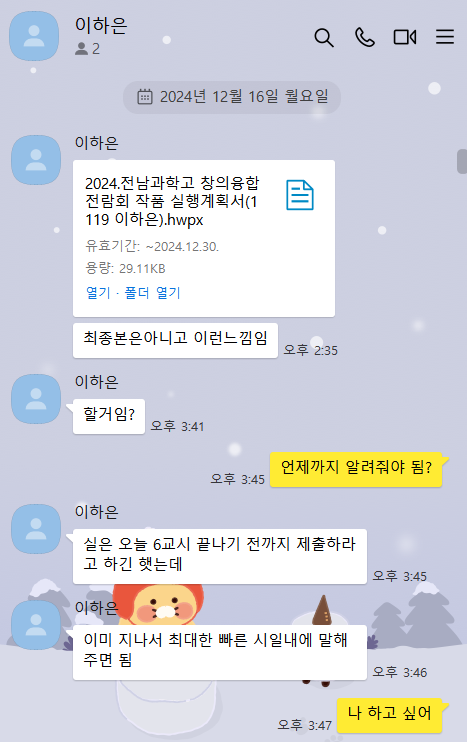
\includegraphics[width=0.45\columnwidth]{4/image07.png}
    \hfill
    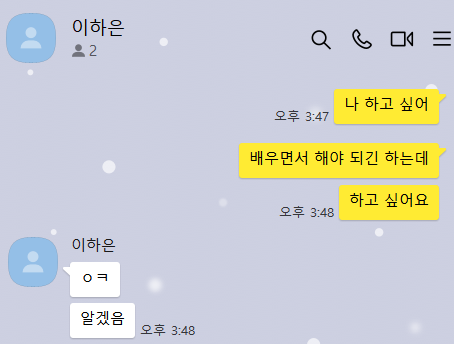
\includegraphics[width=0.45\columnwidth]{4/image08.png}
    \caption{프로젝트 팀 구성}
\end{figure}
팀을 꾸린 이후 방학동안 각자 연구에 필요한 이론을 공부해오기로 했습니다. 
\begin{figure}[h]
    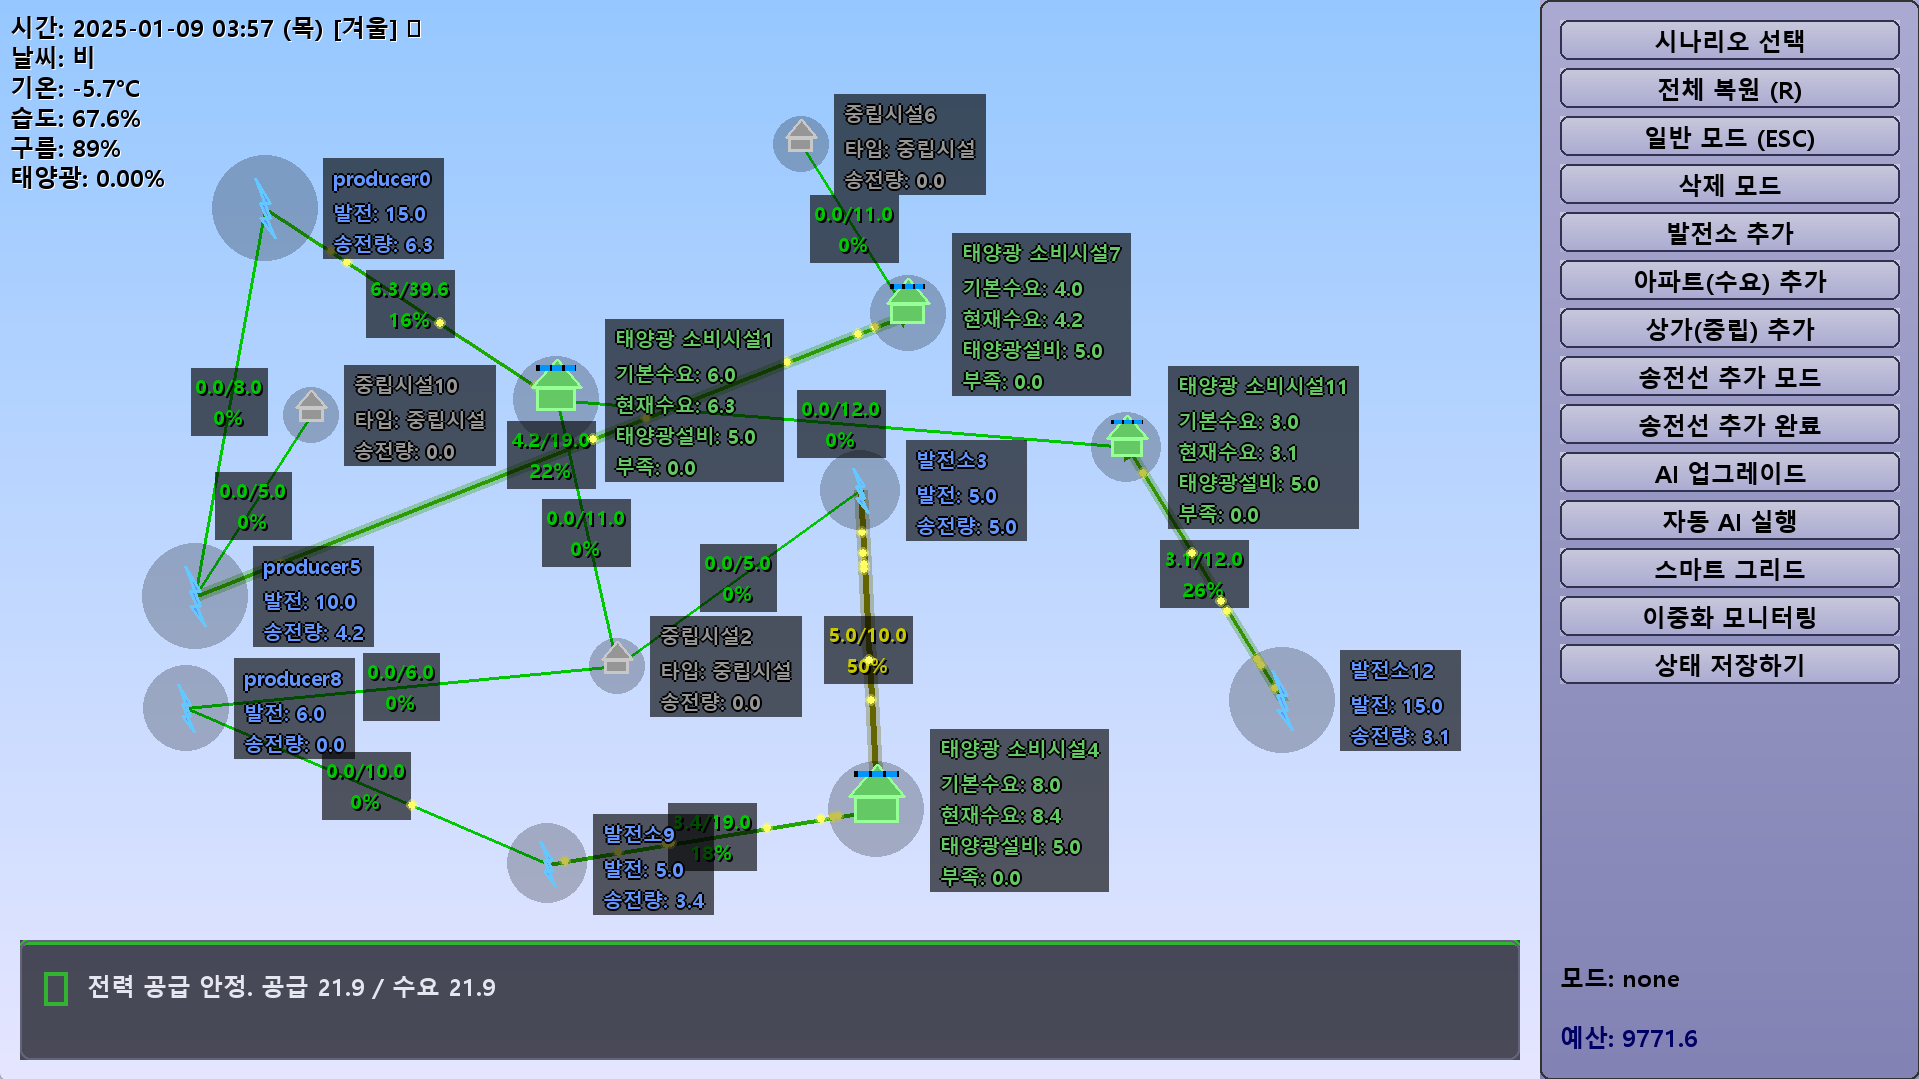
\includegraphics[width=\columnwidth]{4/image09.png}
    \caption{초기 코드 실행 화면}
\end{figure}
\begin{figure}[h]
    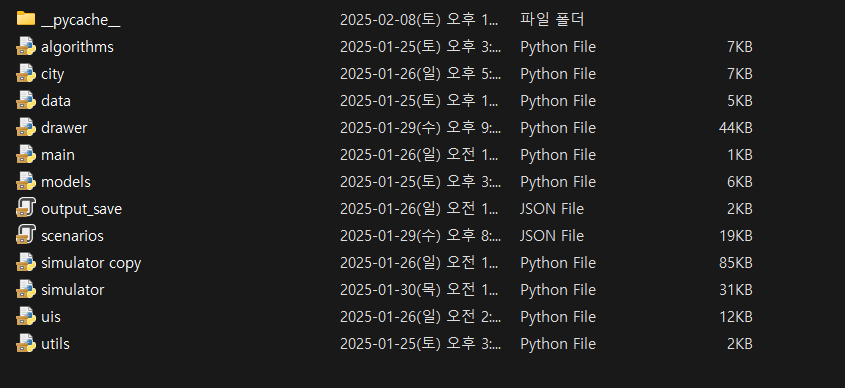
\includegraphics[width=\columnwidth]{4/image10.png}
    \caption{초기 코드 파일 구조}
\end{figure}
저는 공부하면서 초기코드를 작성하였는데, 발전소와 같은 전력 공급원, 주택,아파트와 같은 수요처, 전선  등 대부분의 주요 요소가 구현된 상태였습니다. 원하는 위치에 아파트, 상가, 발전소 등을 배치할 수 있도록 제작했습니다. 폭염 혹은 한파, 자연재해, 발전소 고장 또는 연료 부족, 전력 수급 예측 실패 등 정전 위험 시나리오 일부와 함께 완벽하진 않지만 위험 상황을 자동으로 분석하고 판단해 해결하는 AI도 적용시켰습니다. 
\begin{figure}[h]
    \includegraphics[width=\columnwidth]{4/image.png}
    \caption{시뮬레이터 실행 화면}
\end{figure}
    \label{fig:fsm}
    조원들에게 코드를 공유하는 과정에서도 어려움이 있었습니다.
\subsection{성과}
.

